\section{Background Theories} 

\subsection{Argumentation Theory - Basics}
Fundamental mechanism, humans use in argumentation, and exploring ways to implement this mechanism on computers. 
\begin{itemize}
	\item developing a theory for argumentation (central notion is the acceptability of arguments)
	\item correctness of this theory ( most approaches to nonmonotonic reasoning in AI and logic programming are special forms of this theory of argumentation)
	\item appropriateness of this theory (illustrates how our theory can be used to investigate the logical structure of many practical problems)
\end{itemize}
Mostly based on Dung\cite{Dung1995321}. Biggest difference: we argue with inconsistent SKB so defeasible argumentation. 

Liao \cite[Chapter 2]{liao} provides the same semantic of argumenatation. jsut introducing extension based and labelling based approach. Pointing out difference and 

\subsection{Argumentation Theory - Working with Preferences in AF}
Based on Isabel's second paper\cite{sassoon2016}, based on Extended Argumentation Framework\cite{Modgil2009}, using preferences as arguments for attacks on the attack-relation in the original argumentation.
Distinguishing to Amgouds's\cite{amgoud}  Preference based Argumentation Framework.

\subsection{Source paper}
Short summary of Isabels paper \cite{sassoon2014}. Focus on argumentation theory behind it and model selection process. Preferences expressed as attacks on the attacks between the arguments for models.

\subsection{Related work}
\begin{itemize}
	\item Argumentation for Aggregating Clinical Evidence \cite{hunter}: multiple outcome indicators, checks only old date, not supposed data for recommendation, focuses on generation of arguments out of evidence
	\item An argument-based approach to reasoning with clinical knowledge\cite{Gorogiannis20091}: Focus on simple language representing the results of clinical trials, doesn't deal with preferences of different priorities.
	\item In Argumentation for Decision Support\cite{Atkinson2006} an approach using values in the AF is presented, where $A2$ defeats $A1$ iff $A2$ attacks $A1$ and $val(A2) \ngtr_a val(A1)$ which is not applicable as no strict partial order given.
\end{itemize}


\section{Designprocess - Use Cases}

\begin{itemize}
	\item popular MoSCoW (Must, Should, Could, Would) prioritization scheme
	\item Use Case on one card (Priority, Release, Size, Complexity)
	\item Use Case Slices generated from use case (Flows, Tests, Estimation)
	\item Find Actors and Use Cases (slice them subsequently)
	\item Prepare Use Case Slices by describing related stories (use-case narrative) and defining test cases
	\item Analyse Use Case Slices (check how the system elements will interact to perform the use case)
	\item Implement Use Case Slice
	\item Test Use Case Slice
	\item Inspect and Adapt
	\item Test System
\end{itemize}

\begin{figure}[!ht]
\centering
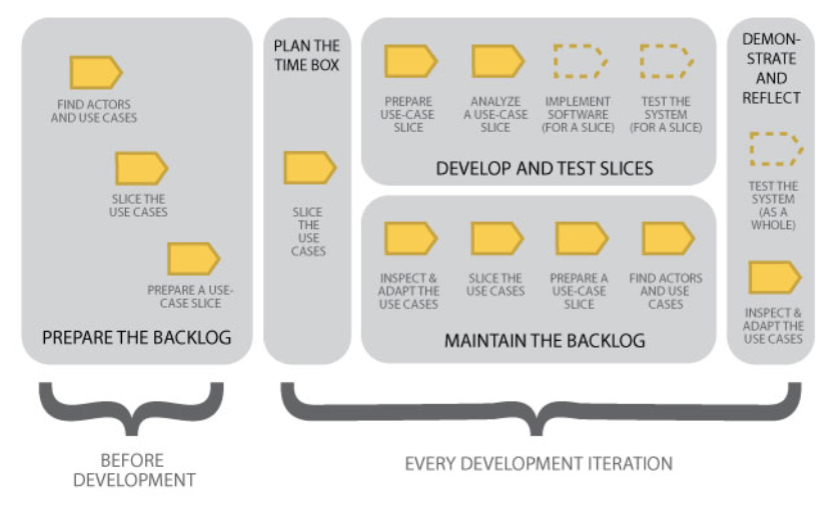
\includegraphics[width=0.8\textwidth]{figures/uc20_flow}
\caption{Use-case 2.0 activities for iterative development approaches}
\label{fig:Pict}
\end{figure}


